\documentclass[11pt,letterpaper,twoside]{article}
\usepackage[english]{babel}
\usepackage{amssymb,amsmath}
\usepackage{fancyhdr}
\usepackage{graphicx}

 \oddsidemargin  0in \evensidemargin 0in
 \topmargin   -0.25in \headheight 0.25in \headsep 0.25in
 \textwidth   6.5in \textheight 8.75in \marginparsep 0pt \marginparwidth 0pt
 \parskip 1ex  \parindent 0ex \footskip 20pt

\newfont{\bssten}{cmssbx10}
\newfont{\bssnine}{cmssbx10 scaled 900}

%%%%%%%%%%%%%%%%%%%%%%%
\newcommand{\whatizit}{Lecture 8: Linear Regression}
%%%%%%%%%%%%%%%%%%%%%%%


\pagestyle{fancy}  
\fancyhead{\bssnine STOR 155,  \whatizit}
\fancyhead[RE]{} \fancyhead[LO]{}
\fancyhead[LE]{\bssnine \thepage} \fancyhead[RO]{\bssnine \thepage}
\lfoot{} \cfoot{} \rfoot{}   


\newcommand{\var}{\mathrm{Var}}



\begin{document}



\thispagestyle{empty} \vspace*{-0.75in}

{\bssten STOR 155: Introduction to Data Models and Inference \hfill May 22, 2024 \\
Prof. Will Lassiter  \hfill Page 1 of \pageref{totalpag}}
\vspace{10pt}
\begin{center} {{\Large \bf \whatizit}} \end{center}

Practice Test Questions: Correlation

\begin{center}
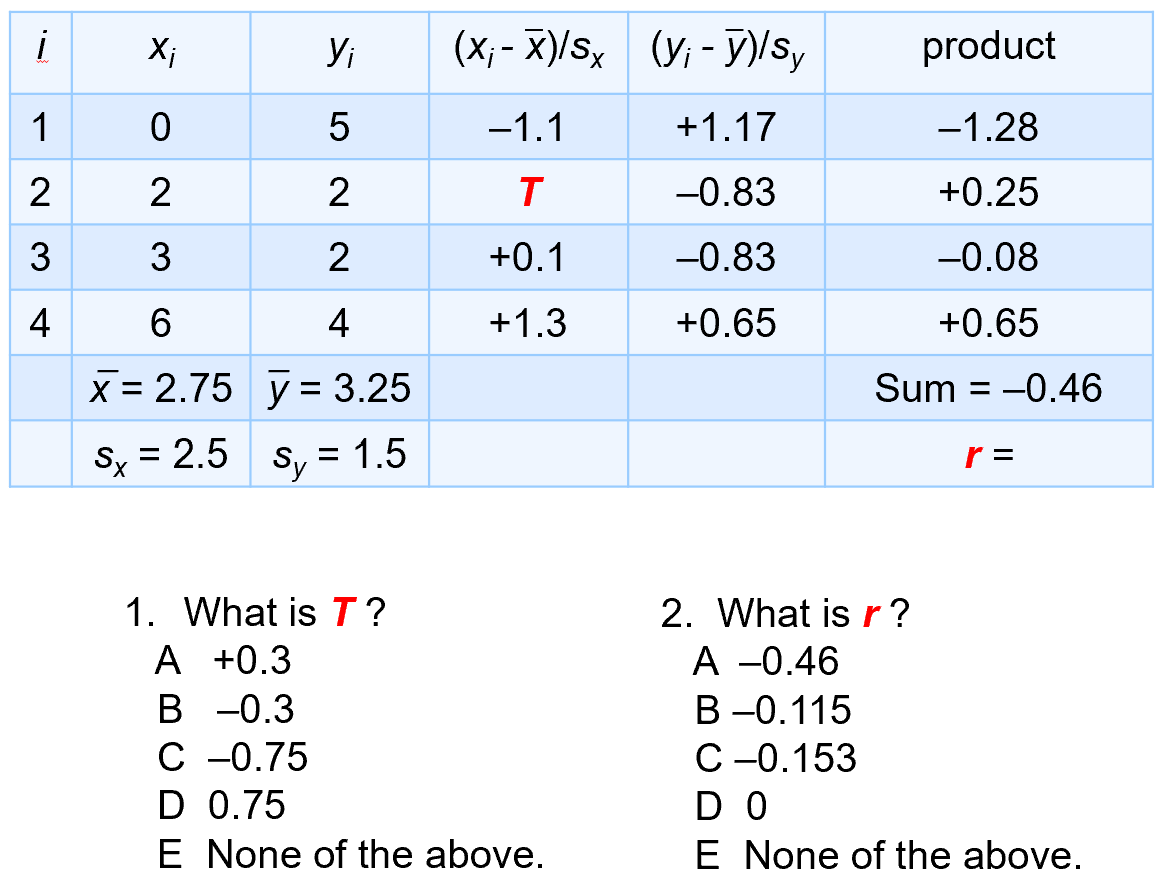
\includegraphics[scale=0.8]{images/correl.png}
\end{center}

\begin{center}
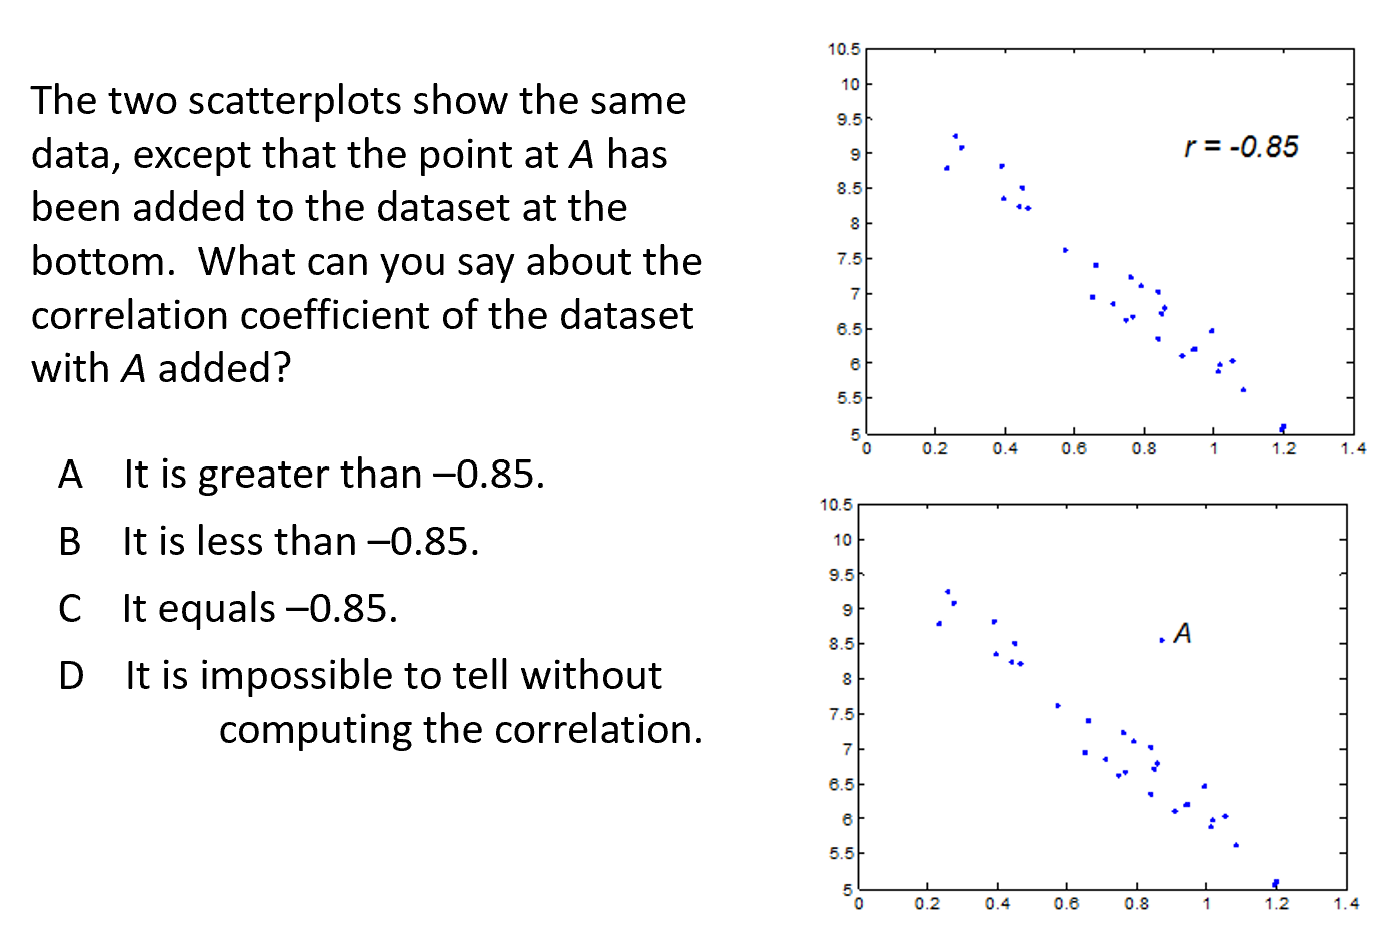
\includegraphics[scale=0.8]{images/correl2.png}
\end{center}

\newpage

{\bf Least Squares Regression} \vspace{6pt}

A {\bf regression line} describes ... \vspace{80pt}

Unlike with correlation, it matters \vspace{40pt}

General equation of a line: \vspace{100pt}

Small example:

\begin{center}
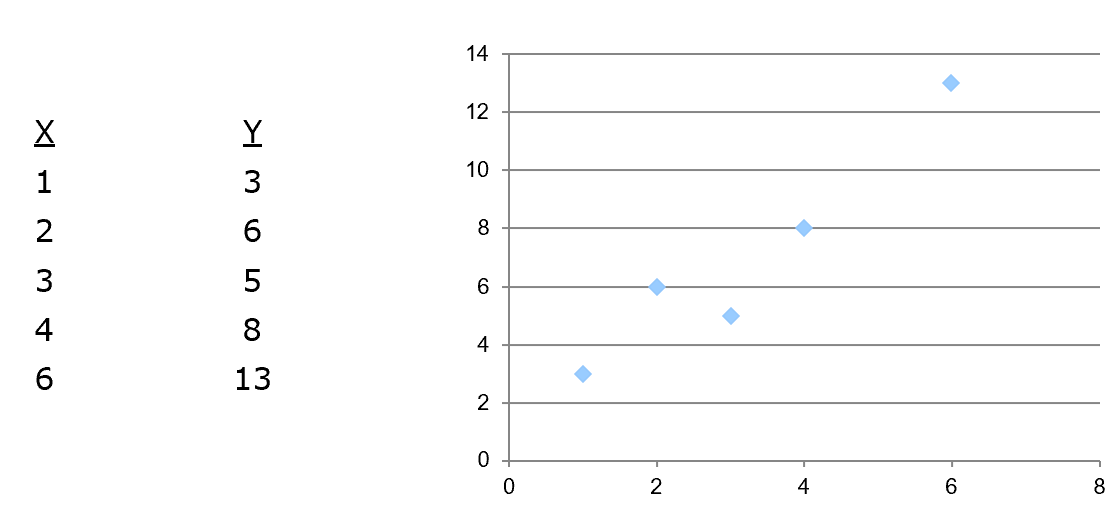
\includegraphics[scale=1]{images/scatter.png}
\end{center}

How to construct a line to fit these data?

\newpage

Notation: \vspace{50pt}

Definition: A {\bf residual} \vspace{50pt}

Mathematically, a least-squares regression line minimizes the sum \vspace{50pt}

What values of $b_0$ and $b_1$ minimize this quantity? \vspace{60pt}

Why the term ``regression"?

\begin{center}
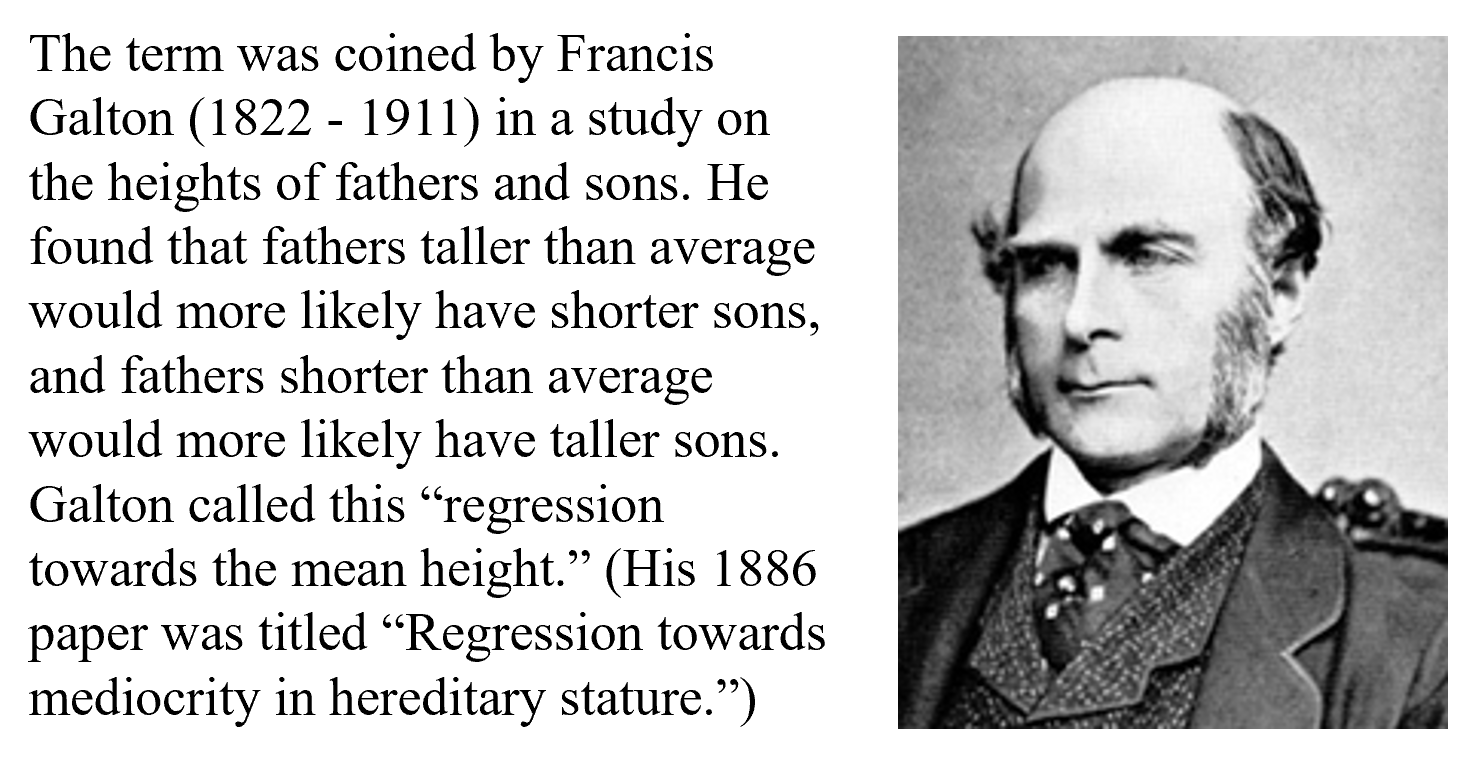
\includegraphics[scale=0.5]{images/galton1.png}
\end{center}

\begin{center}
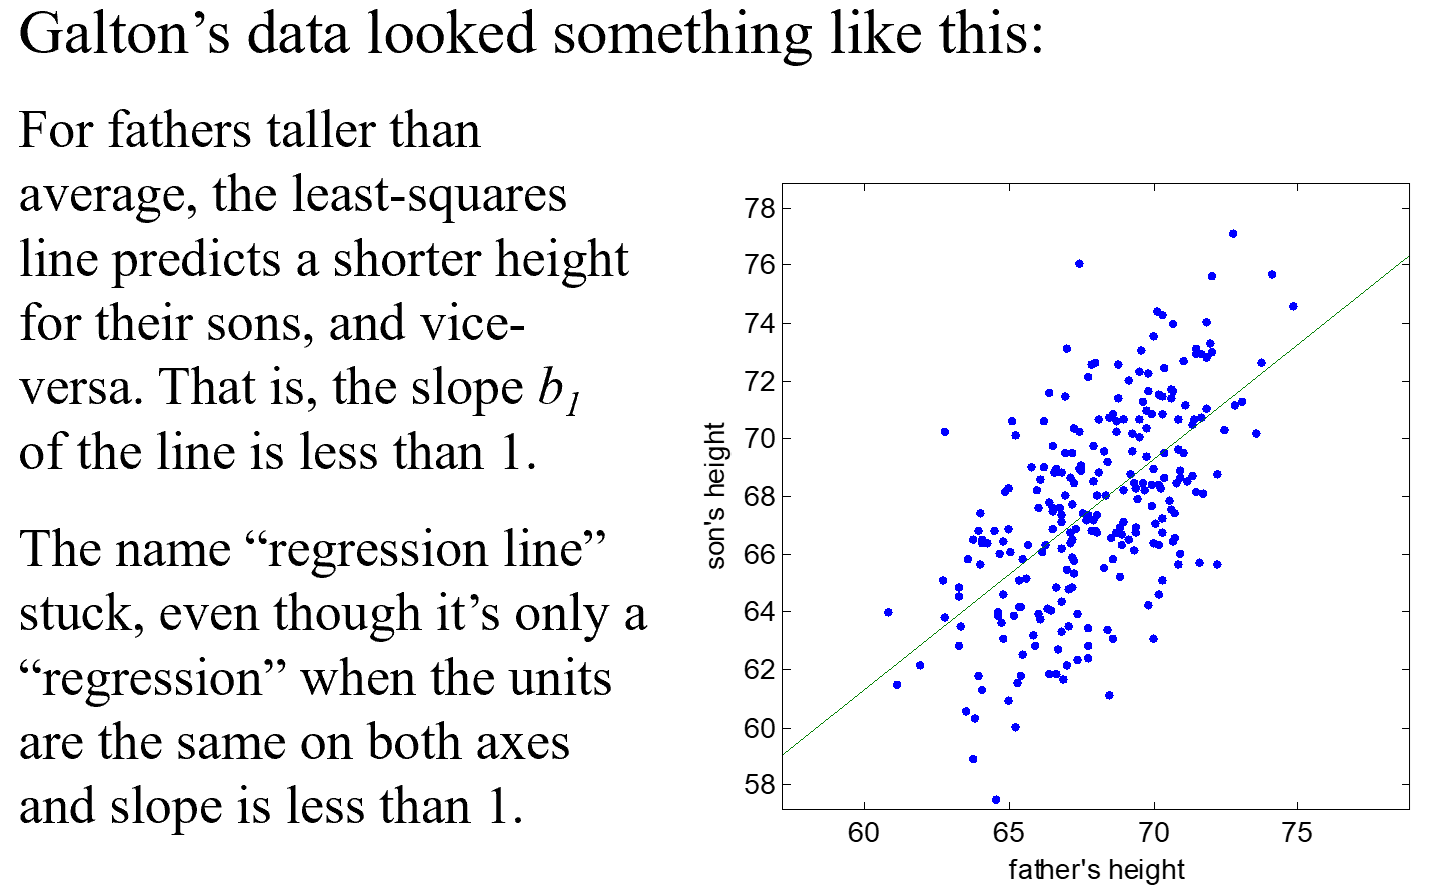
\includegraphics[scale=0.5]{images/galton2.png}
\end{center}

\newpage

Practice: Observations for explanatory  variable $X$ and response variable $Y$ have $$\bar{x}=7, \quad \bar{y}=5, \quad s_x=4, \quad s_y=2, \quad r=0.85$$ Find the equation of a least-squares regression line that we could use to predict an observation of $Y$ given an observation of $X$. \vspace{180pt}


Question: Will switching which variable is explanatory and which is the response change the least-squares line? \vspace{60pt}

Example: Data on galaxies

$X$: galaxy's distance from Earth \\
$Y$: velocity at which galaxy is moving away from Earth

\begin{center}
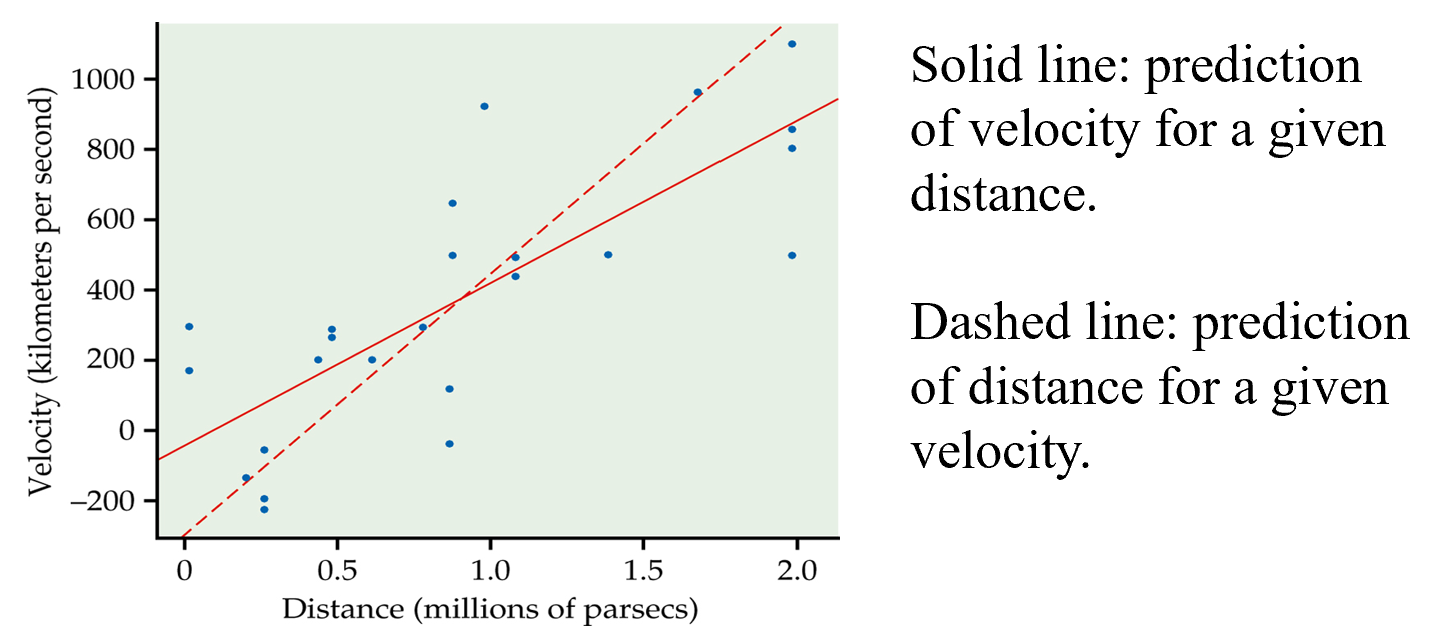
\includegraphics[scale=0.85]{images/galaxy.png}
\end{center}


\newpage

{\bf Connection between Correlation and Regression} \vspace{6pt}

Open the spreadsheet {\tt test\_scores.xlsx} \vspace{10pt}

The value $r^2$ measures ... \vspace{80pt}

Rule of thumb: \vspace{40pt}

\begin{center}
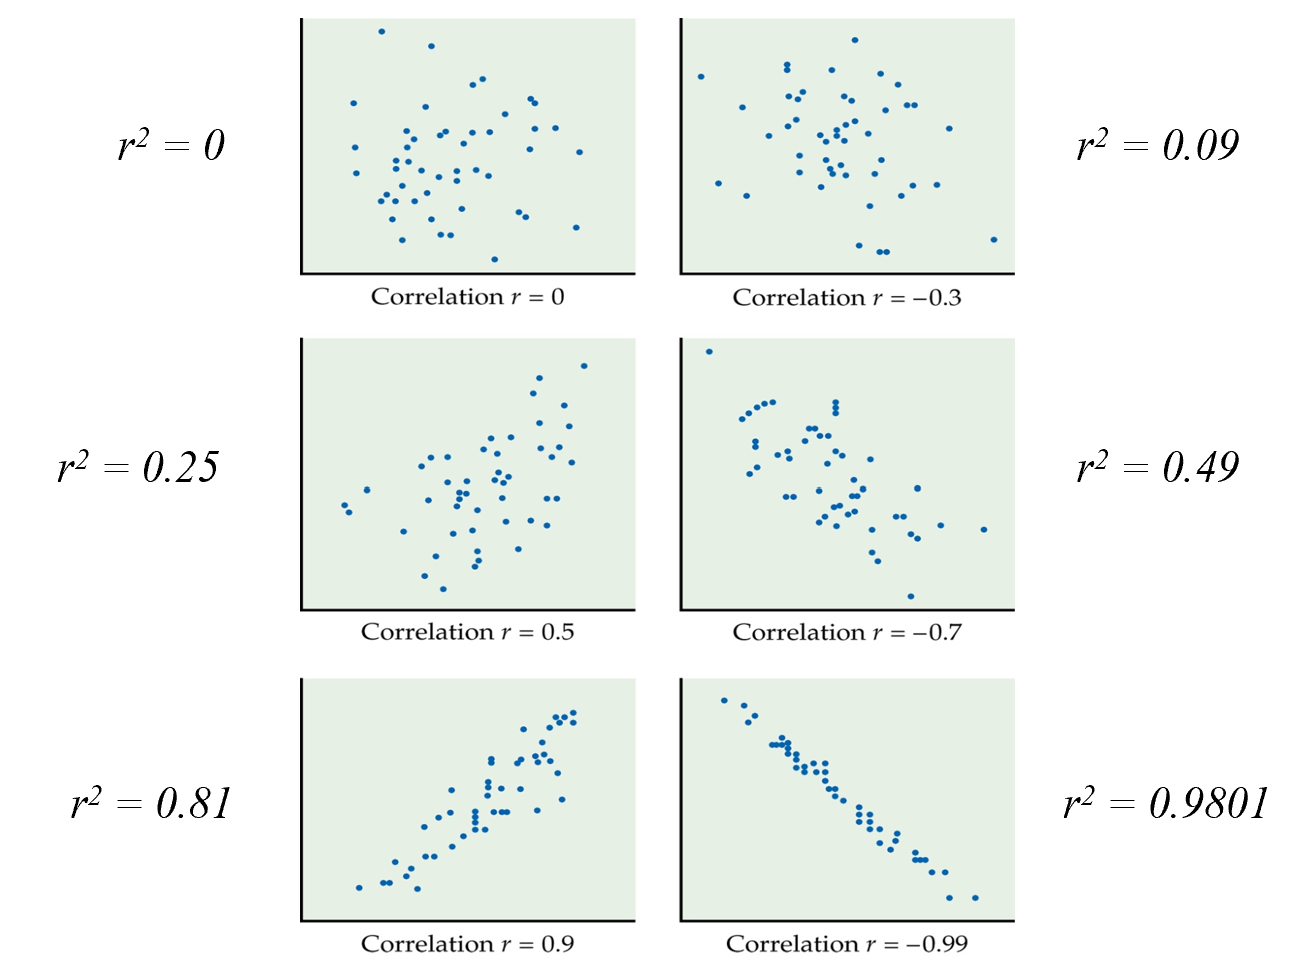
\includegraphics[scale=0.8]{images/rsquared.png}
\end{center}

$r=0.5\implies$ \vspace{60pt}

$r=-0.7\implies$

\newpage

Limitations of using regression to make predictions

\begin{center}
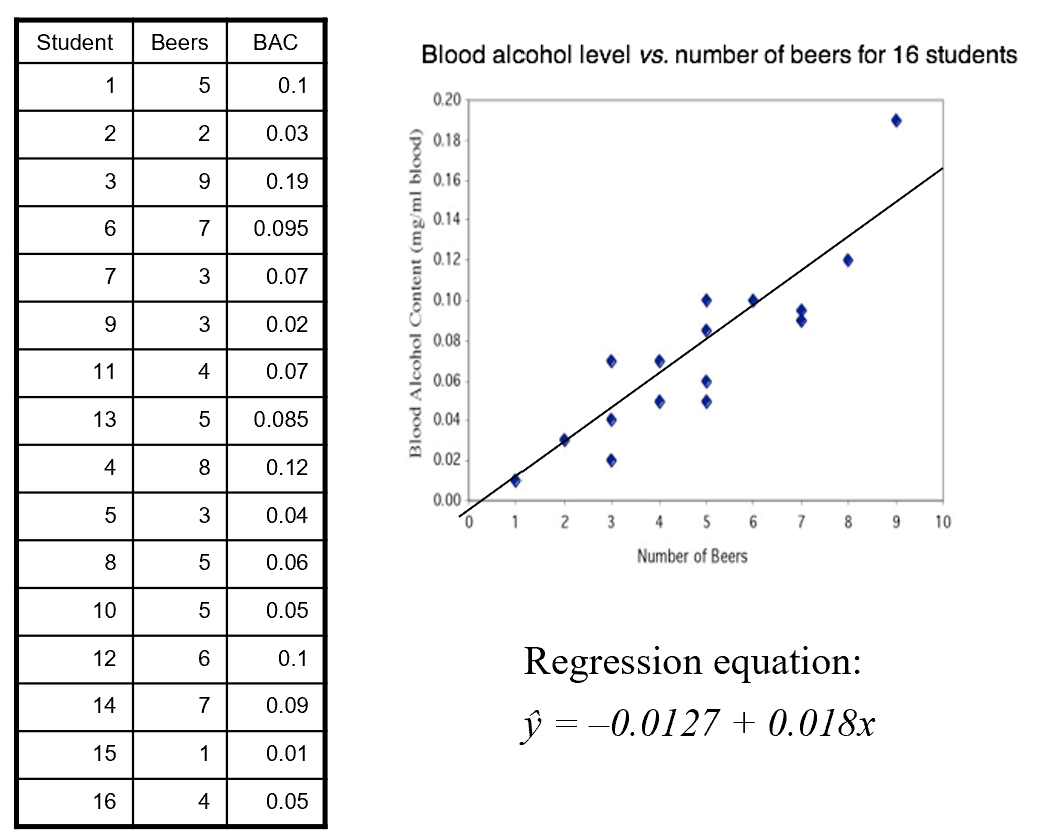
\includegraphics[scale=0.8]{images/beers.png}
\end{center}

Extrapolation vs.\ interpolation: \vspace{180pt}

Practice test question: Researchers measured the two variables below for a large number of subjects.
	
$X =$ sodium intake in mg per day, and \\
$Y =$ systolic blood pressure   

The least-squares regression line for predicting $Y$ given $X$ is
 $$\hat{y} = -15.4 + 2.3x$$   What is the predicted systolic blood pressure for someone whose sodium intake is 60 mg per day?
 
\newpage

{\bf Residual Plots}

\begin{center}
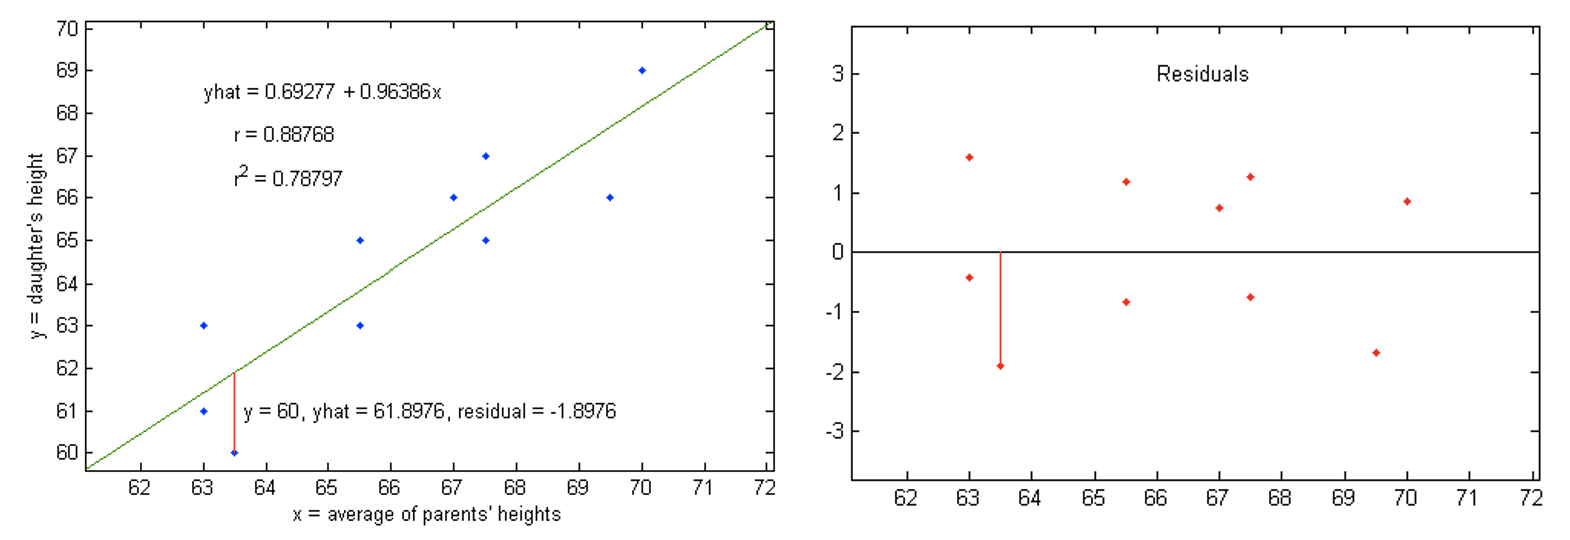
\includegraphics[scale=0.75]{images/residuals1.png}
\end{center}

Why would we want to plot residuals by themselves?

\begin{center}
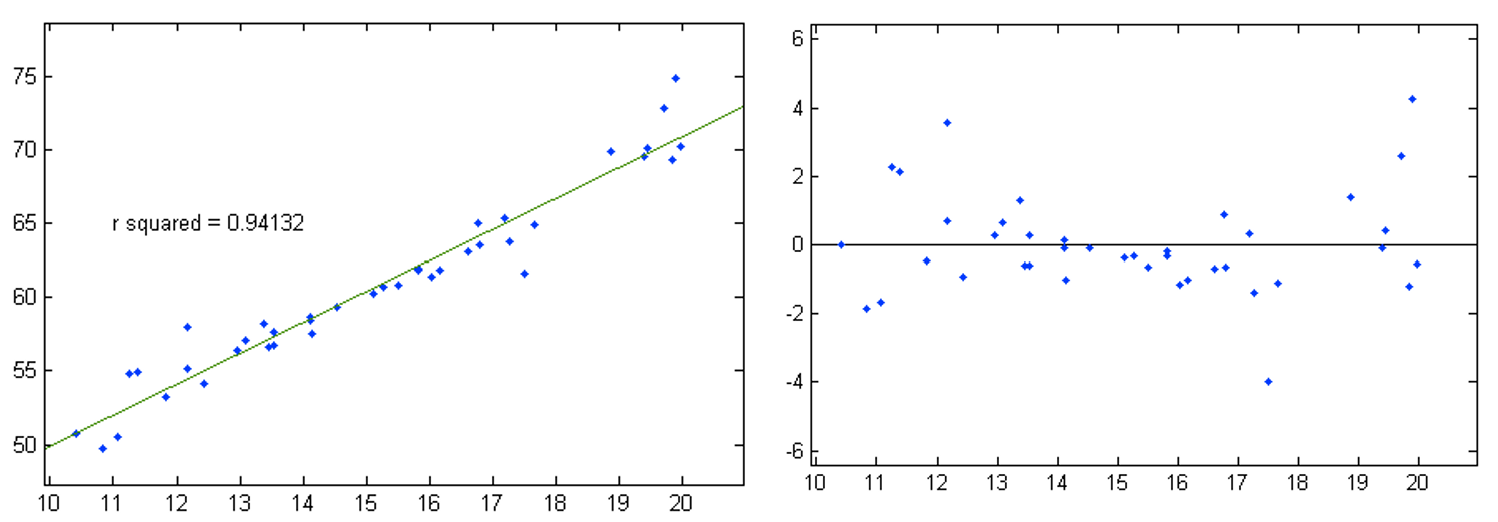
\includegraphics[scale=0.75]{images/residuals2.png}
\end{center}

\vspace{40pt}

Ideal residual plot:

\begin{center}
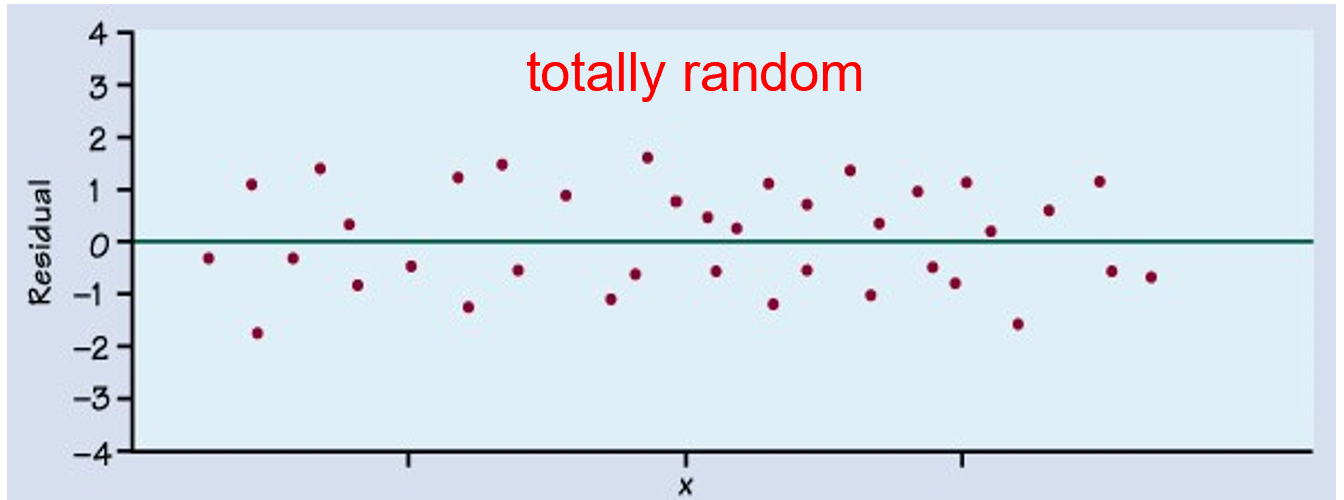
\includegraphics[scale=0.75]{images/residuals3.png}
\end{center}

\newpage

Not-so-ideal residual plots:

\begin{center}
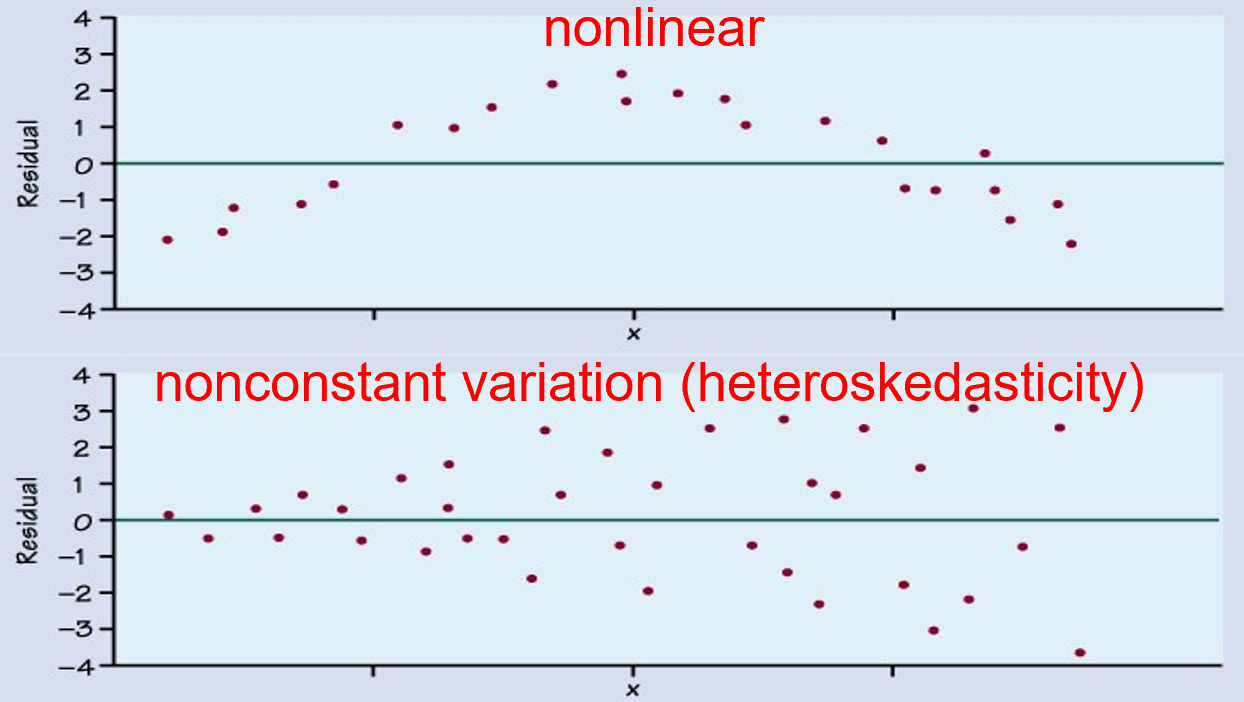
\includegraphics[scale=0.8]{images/residuals4.png}
\end{center}

Influence of outliers:

\begin{center}

\includegraphics[scale=0.75]{images/outliers.png}
\end{center}

\newpage

{\bf Importance of Plotting Data}

\begin{center}
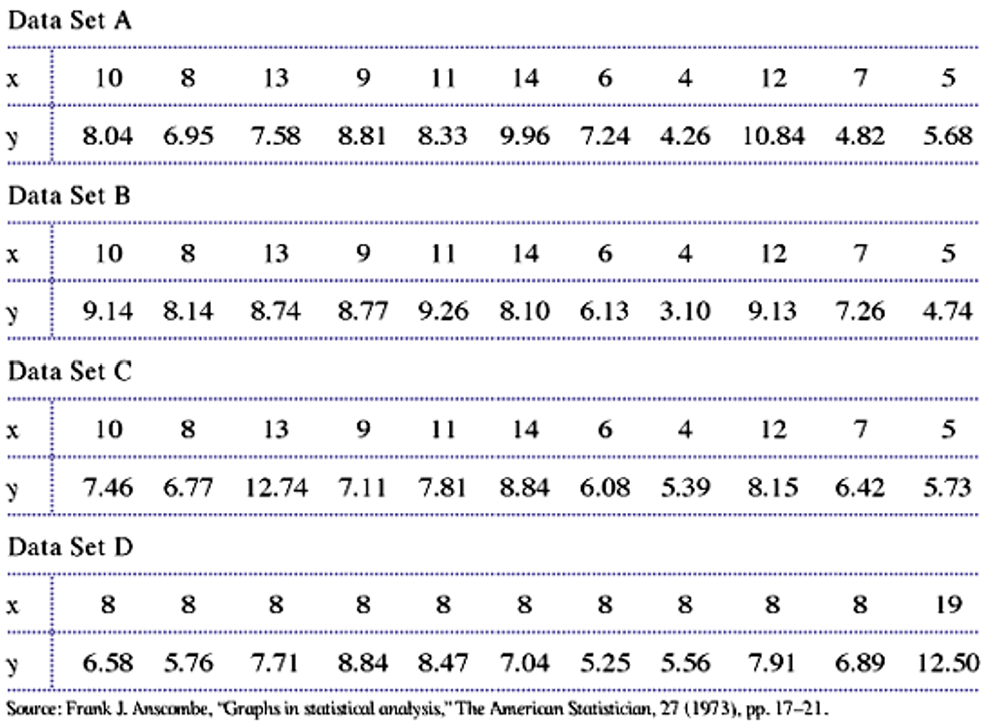
\includegraphics[scale=1]{images/data.png}
\end{center}

All have correlation $r = .816$, regression equation $\hat{y} = 3 + 0.5x$

\begin{center}
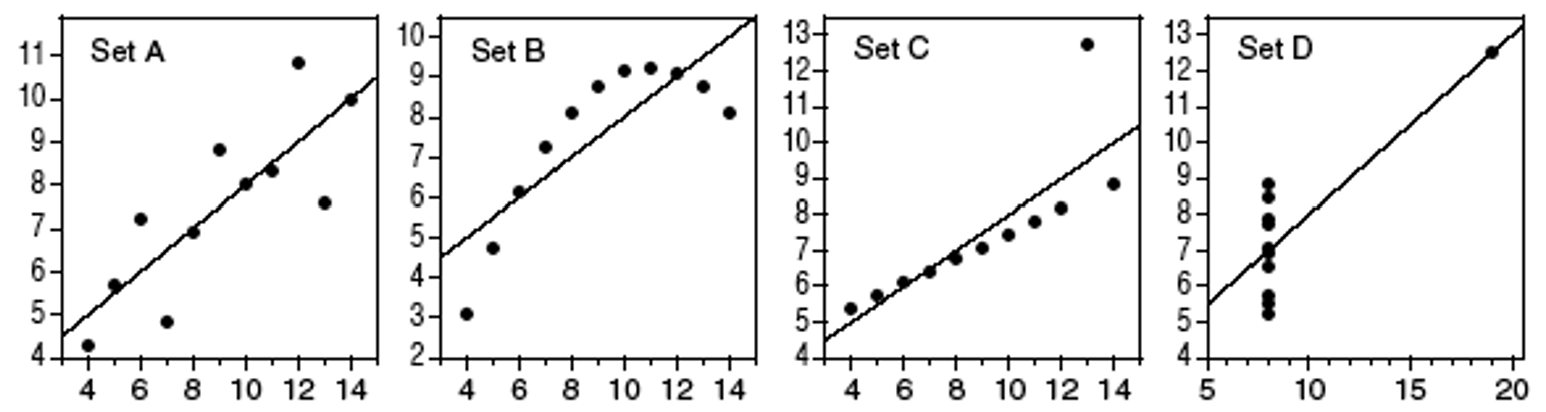
\includegraphics[scale=0.75]{images/data2.png}
\end{center}

\label{totalpag}
\end{document}